\section{Resultados}


%%%%%%%%%%%%%%%%%%%%%%%%%%%%%%%%%%%%%%% Implementação da LPA2v
\begin{frame}{Implementação da LPA2v}

\emph{ P:  eixo do motor apresenta rotação igual ao valor de referência.}

\begin{itemize}
\item $\mu _0$ : grau de evidência favorável que refere-se ao valor desejado;
\item $\mu _1$ : grau de evidência favorável com que o motor atinge a velocidade de rotação desejada;
\end{itemize}
O bloco LPA2v calcula os graus de evidência desfavoráveis das respectivas entradas:

\centering
$\lambda _0 = 1- \mu _0   \hspace{1cm}   \lambda _1 = 1 - \mu_1 $

\vspace{0.5cm}

Para o cálculo dos graus de Certeza e Contradição são utilizados:

\vspace{0.5cm}
\resizebox{!}{0.6cm}{ $ P _{(\mu_0, \lambda_1)} $}


\end{frame}









%%%%%%%%%%%%%%%%%%%%%%%%%%%%%%%%%%%%%%% Diagrama de blocos do Controle utilizando a LPA2v
\begin{frame}{Diagrama de blocos do Controle utilizando a LPA2v}

\begin{figure}[!h]
\centering
%\caption{Diagrama de blocos do controle utilizando a LPA2v}
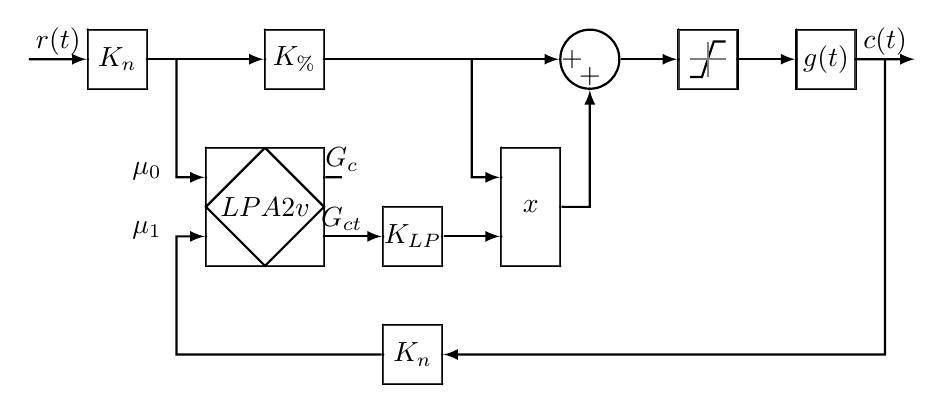
\begin{tikzpicture}[scale=0.75]
\tikzset{ >=latex, inner sep=0pt, outer sep=0pt,  }

%\draw [lightgray, dashed](0,0) grid (15,7);

%%% Blocos 

% K normalização rps -> 0..1
\node [fill=black, circle] (KSP0) at (1,6.5) { };
\node [fill=black, circle] (KSP1) at (2,5.5) { };
\draw[thick] (KSP0) rectangle (KSP1);
\fill[white, nearly transparent] (KSP0) rectangle (KSP1);
\node [fill=black, circle] (KSPin)  at (1.0,6.0) { }; 
\node [fill=black, circle] (KSPout) at (2.0,6.0) { }; 
\node (Kn1) at (1.5,6.0) {$K_n$};

% K normalização  0..1 --> %PWM
\node [fill=black, circle] (KPWM0) at (4,6.5) { };
\node [fill=black, circle] (KPWM1) at (5,5.5) { };
\draw[thick] (KPWM0) rectangle (KPWM1);
\fill[white, nearly transparent] (KPWM0) rectangle (KPWM1);
\node [fill=black, circle] (KPWMin)  at (4.0,6.0) { };
\node [fill=black, circle] (KPWMout) at (5.0,6.0) { };
\node (K100) at (4.5,6.0) {$K_{\%}$};

% Planta
\node [fill=black, circle] (GT0) at (13,6.5) { };
\node [fill=black, circle] (GT1) at (14,5.5) { };
\draw[thick] (GT0) rectangle (GT1);
\fill[white, nearly transparent] (GT0) rectangle (GT1);
\node [fill=black, circle] (GTin)  at (13.0,6.0) { };
\node [fill=black, circle] (GTout) at (14.0,6.0) { };
\node (planta) at (13.5,6.0) {$g(t)$};

% Saturação
\node [fill=black, circle] (SAT0) at (11,6.5) { };
\node [fill=black, circle] (SAT1) at (12,5.5) { };
\draw[thick] (SAT0) rectangle (SAT1);
\fill[white, nearly transparent] (SAT0) rectangle (SAT1);
\node [fill=black, circle] (SATin)  at (11.0,6.0) { };
\node [fill=black, circle] (SATout) at (12.0,6.0) { };
\draw [thick] (11.2,5.7) -- (11.4,5.7) -- (11.6,6.3) -- (11.8,6.3);
\draw [gray, thick] (11.2,6.0) -- (11.8,6.0);
\draw [gray, thick] (11.5,5.7) -- (11.5,6.3);

% Multiplicacao
\node [fill=black, circle] (MUL0) at (8,4.5) { };
\node [fill=black, circle] (MUL1) at (9,2.5) { };
\draw[thick] (MUL0) rectangle (MUL1);
\fill[white, nearly transparent] (MUL0) rectangle (MUL1);
\node [fill=black, circle] (MULin0) at (8.0,4.0) { };
\node [fill=black, circle] (MULin1) at (8.0,3.0) { };
\node [fill=black, circle] (MULout) at (9.0,3.5) { };
\node (multi) at (8.5,3.5) {$x$};

% Klp
\node [fill=black, circle] (KLP0) at (6,3.5) { };
\node [fill=black, circle] (KLP1) at (7,2.5) { };
\draw[thick] (KLP0) rectangle (KLP1);
\fill[white, nearly transparent] (KLP0) rectangle (KLP1);
\node [fill=black, circle] (KLPin)  at (6.0,3.0) { };
\node [fill=black, circle] (KLPout) at (7.0,3.0) { };
\node (KLP) at (6.5,3.0) {$K_{LP}$};

% Sensor
\node [fill=black, circle] (KS0) at (6,1.5) { };
\node [fill=black, circle] (KS1) at (7,0.5) { };
\draw[thick] (KS0) rectangle (KS1);
\fill[white, nearly transparent] (KS0) rectangle (KS1);
\node [fill=black, circle] (KSin)  at (7.0,1.0) { };
\node [fill=black, circle] (KSout) at (6.0,1.0) { };
\node (Kn2) at (6.5,1.0) {$K_n$};

% LPA2v
\node [fill=black, circle] (LPA0) at (3,4.5) { };
\node [fill=black, circle] (LPA1) at (5,2.5) { };
\draw[thick] (LPA0) rectangle (LPA1);
\fill[white, nearly transparent] (LPA0) rectangle (LPA1);
\node [fill=black, circle] (LPAu0) at (3.0,4.0) { };
\node [fill=black, circle] (LPAu1) at (3.0,3.0) { };
\node [fill=black, circle] (LPAgc)  at (5.0,4.0) { };
\node [fill=black, circle] (LPAgct) at (5.0,3.0) { };
\draw [thick] (4.0,4.5) -- (5.0,3.5) -- (4.0,2.5) -- (3.0,3.5) -- (4.0,4.5);
\node (LPA2v) at (4.0,3.5) {$LPA2v$};
\draw [thick] (LPAgc) -- (5.3,4.0);
\node (LPA2vu0)  at (2.0,4.1) {$\mu _0$};
\node (LPA2vu1)  at (2.0,3.1) {$\mu _1$};
\node (LPA2vGc)  at (5.3,4.3) {$G_c$};
\node (LPA2vGct) at (5.3,3.3) {$G_{ct}$};


% Somador
\node [fill=black, circle] (SUM) at (9.5,6.0) { };
\filldraw[fill=white,thick] (SUM) circle (5mm);
\node [fill=black, circle] (SUMin0) at ( 9.0,6.0) { };
\node [fill=black, circle] (SUMin1) at ( 9.5,5.5) { };
\node [fill=black, circle] (SUMout) at (10.0,6.0) { };
\node (Sum0) at (9.2,6.0) {$+$};
\node (Sum1) at (9.5,5.7) {$+$};



%%% Linhas 

% set point
\draw [->, thick] (0.0,6.0) -- (KSPin);
\node (rt) at (0.5,6.3) {$r(t)$};

% setpoint -> normalização %PWM
\draw [->, thick] (KSPout) -- (KPWMin);

% normalização %PWM -> SUM
\draw [->, thick] (KPWMout) -- (SUMin0);

% SUM -> Saturação
\draw [->, thick] (SUMout) -- (SATin);

% Saturação -> GT
\draw [->, thick] (SATout) -- (GTin);

% GT -> fim
\draw [->, thick] (GTout) -- (15,6);
\node (ct) at (14.5,6.3) {$c(t)$};

% LPA2v Gct -> KLP
\draw [->, thick] (LPAgct) -- (KLPin);

% KLP -> MULin1
\draw [->, thick] (KLPout) -- (MULin1);

% normalização 0..1 -> LPA2v u0
\draw [->, thick] (2.5,6.0) -- (2.5,4.0) -- (LPAu0);

% normalização %PWM -> MULT in0
\draw [->, thick] (7.5,6.0) -- (7.5,4.0) -- (MULin0);

% MULT out -> SUM in1
\draw [->, thick] (MULout) -- (9.5,3.5) -- (SUMin1);

% Fim -> sensor
\draw [->, thick] (14.5,6.0) -- (14.5,1.0) -- (KSin);

% Sensor -> LPA u2
\draw [->, thick] (KSout) -- (2.5,1.0) -- (2.5,3.0) --(LPAu1);

\end{tikzpicture}
\label{fig:diagramaBlocosLPA2v}

%{\vspace{0.2cm} \small Fonte: Próprio autor}
\end{figure}


\end{frame}


%%%%%%%%%%%%%%%%%%%%%%%%%%%%%%%%%%%%%%% Descrição do diagrama
\begin{frame}{Descrição do diagrama de blocos}


\begin{itemize}
  \item $K_n$: Bloco de normalização: rps para um intervalo fechado entre 0,0 e 1,0;

  \item $K_{\%}$: Bloco de normaliza: intervalo fechado entre 0,0 e 1,0 para um intervalo de 0 a 100 (\%PWM);

  \item $LPA2v$: Calcula os graus de Certeza e Contradição 
de acordo com os graus de evidência favorável $\mu _0$ e $\mu _1$;

  \item $K_{LP}$: Coeficiente de ganho proporcional do grau de contradição;

  \item $x$: Bloco multiplicador;

  \item $g(t)$: Planta do sistema;

  \item $Soma$: Bloco somador;

  \item \emph{Saturação}: Bloco limitador, impede o valor do PWM ultrapassar seu valor máximo de 100\%. 
\end{itemize}



\end{frame}



%%%%%%%%%%%%%%%%%%%%%%%%%%%%%%%%%%%%%%% Ação de Controle utilizando LPA2v
\begin{frame}{Ação de Controle utilizando LPA2v}

\begin{figure}[!htb]
%\caption{Ação de controle utilizando LPA2v}
\vspace{-1cm}\center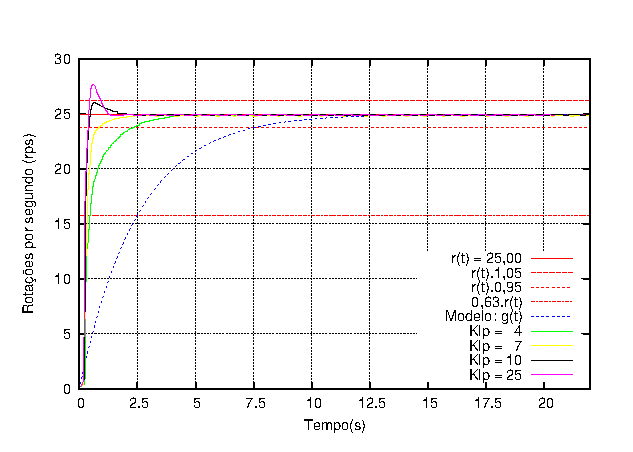
\includegraphics[scale=1.0]{./imagens/klpAll.eps}
\label{fig:acaoLPA2v}

%{\small Fonte: Próprio autor}
\end{figure}


\end{frame}



%%%%%%%%%%%%%%%%%%%%%%%%%%%%%%%%%%%%%%% Ação de Controle utilizando LPA2v
\begin{frame}{Ação de Controle utilizando LPA2v}


\begin{figure}[!htb]
%\caption{Ação de controle utilizando LPA2v para valores alvo variáveis}
\vspace{-1cm}
\center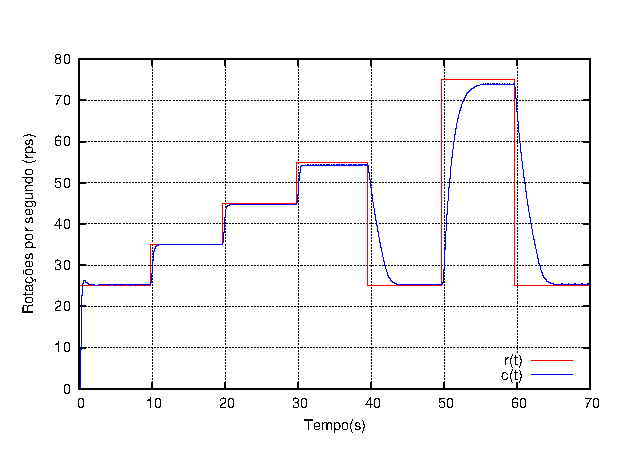
\includegraphics[scale=1.0]{./imagens/patam85.eps}
\label{fig:acaoLPA2vpatam85}

%{\small Fonte: Próprio autor}
\end{figure}

\end{frame}

